\section{Evaluation}
\label{sec:eval}
\label{sec:experiments}

We evaluate document-level KG repair under two complementary protocols. A
controlled paired benchmark provides exact defect provenance and supports
per-defect statistical tests. A separate extraction benchmark contains errors
that arise from a real text-to-graph call rather than from an injection
procedure. We then isolate the simple-pipeline, constraint, routing,
cross-model, cross-domain, and scaling effects.

\subsection{Experimental Protocol}
\label{sec:eval:setup}

\paragraph{Source records and controlled pairs.}
The source corpora contain 4,728 government-affairs records from the Shaanxi
Provincial Government website, 1,000 financial-regulation records from the
National Financial Regulatory Administration, and 500
environmental-regulation records from the Ministry of Ecology and
Environment. We sample up to 500 documents per domain and construct a small
field-level KG for each document. Documents are assigned by source identity to
train, validation, and test groups with a 70/15/15 split and seed 42 before
corruption, preventing clean/corrupted variants from crossing partitions.

Each controlled instance receives exactly two effective changes selected from
six classes: missing triple, duplicate triple, invalid relation, reversed edge,
unsupported value, and hierarchy conflict. The manifest records every clean
and corrupted triple. The held-out split contains 225 documents, balanced at
75 per domain, and 450 manifested defects (Table~\ref{tab:repair_benchmark}).
This protocol measures known repair obligations; it does not estimate their
natural prevalence.

\begin{table}[t]
\centering
\caption{Controlled paired benchmark. Counts in the last three columns are documents.}
\label{tab:repair_benchmark}
\small
\begin{tabular}{l r r r r r}
\toprule
Domain & Documents & Defects & Train & Val. & Test \\
\midrule
Government & 499 & 998 & 349 & 75 & 75 \\
Finance & 500 & 1,000 & 350 & 75 & 75 \\
Environment & 500 & 1,000 & 350 & 75 & 75 \\
\midrule
Total & 1,499 & 2,998 & 1,049 & 225 & 225 \\
\bottomrule
\end{tabular}
\end{table}

\paragraph{Natural extraction errors.}
For the same 225 held-out sources, a fresh Claude Haiku call receives only the
source text, required document node, and relation vocabulary and constructs a
graph from scratch. It never sees the structured target, a corrupted graph, or
the injection manifest. The structured source fields define the reference
graph. Thus, discrepancies are produced by an actual extraction run and are
not selected from predefined defect templates. Ten malformed JSON responses
are retained as empty end-to-end outputs. Overall parse success is 95.56\%; 77
of 225 output graphs differ from the reference, with 302 multiset triple
discrepancies. This is a structured-reference evaluation; two-annotator human
adjudication of acceptable alternatives is not claimed.

\paragraph{Compared repair methods.}
All methods receive the same input graph, source evidence, required document
node, and relation vocabulary.
\begin{itemize}
    \item \textbf{No Repair} returns the input unchanged.
    \item \textbf{Rule Only} deduplicates, reverses an edge when its object is
    the required document node, and removes invalid heads or relations.
    \item \textbf{SHACL-style Repair} applies canonical-head and
    allowed-predicate shapes \citep{ref_shacl2017}; it cannot reconstruct
    missing values from text.
    \item \textbf{Direct LLM} makes one source-grounded call and returns a
    complete graph.
    \item \textbf{ReAct-style Agent} makes a diagnosis call followed by an
    action call \citep{ref_yao2023react}.
    \item \textbf{Simple Pipeline} applies the same deterministic
    preprocessing as the full system, makes one source-grounded call, and only
    deduplicates the response. It has no quality profile, learned prior,
    trial-state utility, or constraint gate.
    \item \textbf{Full System} uses profile-conditioned completion and rejects
    invalid-head, invalid-relation, unsupported, duplicate, and
    relation-cardinality proposals.
\end{itemize}

Unless stated otherwise, model-backed methods use the same served
\texttt{claude-haiku-4-5-20251001} checkpoint \citep{ref_anthropic_claude45},
temperature zero, and endpoint. Failures remain in the denominator. On the
controlled set, Direct LLM and Simple Pipeline each have one malformed JSON
response; the Full System and ReAct have none.

\paragraph{Metrics and statistics.}
On the controlled benchmark, defect repair requires restoration of the clean
triple multiplicity and removal of its corrupted form. We also report
clean-fact preservation, over-repair, triple F1, exact multiset graph match,
calls, and latency. For a naturally extracted input $G_0$, output $G_1$, and
reference $G^*$, let $d$ be multiset symmetric-difference size. Natural-error
reduction is
\[
    1-\frac{d(G_1,G^*)}{d(G_0,G^*)},
\]
averaged over the 77 non-exact inputs; negative values mean that repair adds
more errors than it removes. Confidence intervals use 10,000 paired bootstrap
resamples for the new comparisons. Defect outcomes and exact graph matches use
exact McNemar tests; the natural error-count comparison additionally uses a
one-sided paired Wilcoxon test.

\subsection{Controlled Repair Results}
\label{sec:eval:overall}

Table~\ref{tab:repair_main} shows that the Full System repairs 98.00\% of
defects, preserves 99.32\% of clean facts, and reaches 99.17\% triple F1. The
strong Simple Pipeline reaches 95.11\% repair and 96.34\% F1 under the same
one-call budget. The Full System uniquely repairs 15 defects missed by the
Simple Pipeline, while the reverse occurs twice (exact McNemar
$p=0.00235$). Its gain therefore remains after introducing the strongest
implementation-matched baseline, although that baseline closes much of the
gap over Direct LLM.

\begin{table*}[t]
\centering
\caption{Controlled held-out results over 225 documents and 450 defects. Higher is better except for over-repair, calls, and latency.}
\label{tab:repair_main}
\small
\resizebox{\textwidth}{!}{%
\begin{tabular}{l c c c c c c c}
\toprule
Method & Defect repair & Preservation & Over-repair & Triple F1 & Exact match & Calls/doc & Latency/doc \\
\midrule
No Repair & 0.0000 & \textbf{1.0000} & \textbf{0.0000} & 0.7615 & 0.0000 & 0.00 & $<0.001$ s \\
Rule Only & 0.3200 & \textbf{1.0000} & \textbf{0.0000} & 0.8472 & 0.0622 & 0.00 & $<0.001$ s \\
SHACL-style Repair & 0.0000 & \textbf{1.0000} & \textbf{0.0000} & 0.7998 & 0.0000 & 0.00 & $<0.001$ s \\
Direct LLM & 0.9244 & 0.9687 & 0.0758 & 0.9520 & 0.8267 & 1.00 & 7.25 s \\
ReAct-style Agent & 0.8911 & 0.9324 & 0.1667 & 0.9213 & 0.5956 & 2.00 & 20.50 s \\
Simple Pipeline & 0.9511 & 0.9723 & 0.0705 & 0.9634 & 0.8400 & 1.00 & 9.27 s \\
\textbf{Full System} & \textbf{0.9800} & 0.9932 & 0.0167 & \textbf{0.9917} & \textbf{0.9333} & 1.00 & 11.44 s \\
\bottomrule
\end{tabular}%
}
\end{table*}

The Full System succeeds on 28 defects missed by Direct LLM versus three in the
opposite direction ($p=4.65\times10^{-6}$), and on 42 missed by ReAct versus
two in the opposite direction ($p=1.13\times10^{-10}$). These tests concern
the controlled defect distribution.

\begin{figure*}[t]
\centering
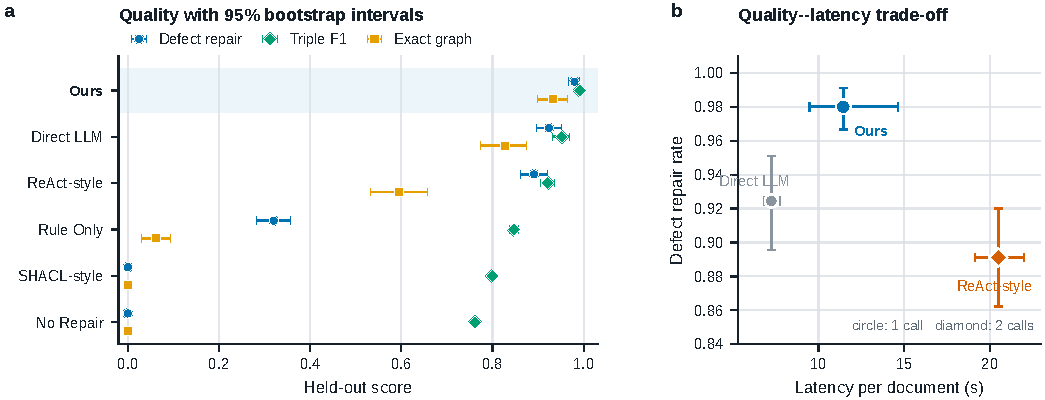
\includegraphics[width=0.98\textwidth]{figure/experiments/repair_benchmark_results.pdf}
\caption{Controlled repair results. \textbf{a}, Defect repair, triple F1, and exact graph match with 95\% document-bootstrap intervals. \textbf{b}, Quality--latency trade-off for one- and two-call model-backed methods.}
\label{fig:repair_benchmark_results}
\end{figure*}

\subsection{Naturally Occurring Extraction Errors}
\label{sec:eval:natural}

Table~\ref{tab:natural_errors} provides the main external-validity check. The
unrepaired extraction output has 87.99\% F1 and 65.78\% exact match. The Simple
Pipeline changes few exact-match outcomes, but its mean error reduction on the
77 imperfect inputs is $-59.15\%$: aggressive completion introduces more
reference disagreements than it removes. In contrast, the Full System reduces
errors by 27.75\%, preserves every initially correct fact on average, and
raises F1 to 92.48\%. Its paired F1 advantage over the Simple Pipeline is 4.40
points (95\% CI: 3.07--5.77), and it prevents 1.03 errors per document on
average (95\% CI: 0.77--1.32; one-sided Wilcoxon
$p=3.18\times10^{-12}$). Exact-match discordance is only three versus zero
and is not significant ($p=0.25$), so the evidence is stronger for partial
graph quality than for complete recovery.

\begin{table*}[t]
\centering
\caption{Repair of graphs produced by an actual extraction call. Error reduction is averaged over the 77 non-exact inputs; other quality metrics use all 225 documents.}
\label{tab:natural_errors}
\small
\resizebox{\textwidth}{!}{%
\begin{tabular}{l c c c c c c c}
\toprule
Method & Parse & Docs with errors & Error reduction & Preservation & Over-repair & Triple F1 & Exact match \\
\midrule
Extracted graph, no repair & 0.9556 & 77 & 0.0000 & 1.0000 & 0.0000 & 0.8799 & 0.6578 \\
Simple Pipeline & 1.0000 & 77 & $-0.5915$ & 0.9971 & 0.2389 & 0.8807 & 0.6711 \\
\textbf{Full System} & 0.9956 & 77 & \textbf{0.2775} & \textbf{1.0000} & \textbf{0.0292} & \textbf{0.9248} & \textbf{0.6844} \\
\bottomrule
\end{tabular}%
}
\end{table*}

\subsection{Component and Constraint-Gate Analysis}
\label{sec:eval:ablation}

The archived ablations reuse the same held-out run. Removing contextual
reasoning leaves deterministic preprocessing; removing preprocessing is the
same one-pass setting as Direct LLM; and removing the gate evaluates the exact
stored pre-gate proposal without another model call.

\begin{table}[t]
\centering
\caption{Controlled component ablation.}
\label{tab:repair_ablation}
\small
\begin{tabular}{l c c c c}
\toprule
Variant & Repair & Over-repair & F1 & Exact \\
\midrule
No context reasoning & 0.3200 & 0.0000 & 0.8472 & 0.0622 \\
No structural preprocessing & 0.9244 & 0.0758 & 0.9520 & 0.8267 \\
No constraint gate & 0.9800 & 0.0227 & 0.9895 & 0.9333 \\
\textbf{Full System} & \textbf{0.9800} & \textbf{0.0167} & \textbf{0.9917} & \textbf{0.9333} \\
\bottomrule
\end{tabular}
\end{table}

Contextual reasoning supplies most recovery, and structural preprocessing
raises F1 by 3.97 points over Direct LLM. The gate does not increase the number
of repaired manifested defects in this run, but lowers over-repair by 0.60
points. A proposal-level audit makes this role concrete: the gate rejects eight
triples, all for absent source support, and all eight are non-reference facts;
it rejects no reference triple. This supports a conservative validation claim,
not a claim that the gate creates missing facts.

\subsection{Actual Router-Controlled Execution}
\label{sec:eval:router}

We compare the learned MLP with violation-based, quality-threshold, random,
always-repair, and never-repair policies. For every routed item, the table uses
the archived full-system output, call count, and measured latency; skipped
items return their input. Clean inputs were executed through the full system in
a separate 225-case run. The resulting costs are therefore assembled from
actual route and repair outcomes rather than projected by multiplying a repair
cost by a routing fraction.

On the balanced controlled stream, the learned, violation, and threshold
policies all obtain routing F1 1.000, 99.59\% triple F1, and 0.50 calls per
document. On the natural stream, they again make identical decisions: routing
F1 is 0.842, with no false positives but a 27.27\% false-negative rate. They
use 0.124 calls per document and retain 96.15\% triple F1. The learned router
therefore does not outperform transparent policies under the evaluated
features. We retain it as an optional policy implementation rather than a
headline source of quality gain.

\begin{table*}[t]
\centering
\caption{End-to-end routing on the 450-item natural stream (225 clean reference graphs plus 225 extraction outputs).}
\label{tab:router_e2e}
\small
\resizebox{\textwidth}{!}{%
\begin{tabular}{l c c c c c c}
\toprule
Policy & Route F1 & FN rate & FP rate & Triple F1 & Exact match & Calls/doc \\
\midrule
Always repair & 0.292 & 0.000 & 1.000 & 0.9582 & 0.8244 & 1.000 \\
Learned router & 0.842 & 0.273 & 0.000 & \textbf{0.9615} & \textbf{0.8422} & 0.124 \\
Violation heuristic & 0.842 & 0.273 & 0.000 & \textbf{0.9615} & \textbf{0.8422} & 0.124 \\
Quality threshold & 0.842 & 0.273 & 0.000 & \textbf{0.9615} & \textbf{0.8422} & 0.124 \\
Random 50\% & 0.242 & 0.532 & 0.493 & 0.9429 & 0.8222 & 0.489 \\
Never repair & 0.000 & 1.000 & 0.000 & 0.9400 & 0.8289 & 0.000 \\
\bottomrule
\end{tabular}
}
\end{table*}

A leave-one-domain-out retraining check uses two domains for training and the
third for testing. Trigger F1 is 1.000 for environment and finance and 0.999
for government; scope-prior top-1 is 1.000 in all three runs. Because these
labels still come from controlled corruptions, the result demonstrates domain
transfer of that mapping rather than natural-error generalization.

\subsection{Cross-Model Robustness}
\label{sec:eval:crossmodel}

We rerun Direct LLM, Simple Pipeline, and Full System on a fixed 60-case subset
(20 per domain) with Claude Haiku and
\texttt{google/gemma-4-26B-A4B-it} \citep{ref_gemma4}. Inputs, prompts,
temperature, and one-call budgets are held fixed. Table~\ref{tab:cross_model}
shows that the Full System has the highest repair rate with both models. Its
absolute F1 advantage over the Simple Pipeline is larger with Claude; Gemma's
stronger direct outputs leave less room for post-processing.

\begin{table}[t]
\centering
\caption{Cross-model controlled results on the same 60 cases.}
\label{tab:cross_model}
\small
\begin{tabular}{l l c c c}
\toprule
Model & Method & Repair & F1 & Exact \\
\midrule
Claude & Direct & 0.958 & 0.970 & 0.867 \\
Claude & Simple & 0.958 & 0.966 & 0.833 \\
Claude & \textbf{Full} & \textbf{0.975} & \textbf{0.991} & \textbf{0.917} \\
\midrule
Gemma & Direct & 0.958 & 0.988 & 0.883 \\
Gemma & Simple & 0.967 & 0.984 & 0.867 \\
Gemma & \textbf{Full} & \textbf{0.983} & \textbf{0.990} & \textbf{0.917} \\
\bottomrule
\end{tabular}
\end{table}

\subsection{Profile Scaling and Incremental Updates}
\label{sec:eval:scale}

The deployed eight-feature routing profile uses exact duplicate, schema,
missing-field, and source-support counts. We form disjoint batches from real
document graphs, assigning unique identifiers when the corpus must be repeated,
and evaluate 1K--50K triples. Full-profile times are medians of seven CPU runs;
one-document incremental times are medians of 200 runs. These measurements do
not include an LLM call or the quadratic semantic-similarity variant in
Eq.~(\ref{eq:q_uniq}).

\begin{table}[t]
\centering
\caption{Measured routing-profile scaling.}
\label{tab:profile_scaling}
\small
\begin{tabular}{r r r r r}
\toprule
Triples & Documents & Full (ms) & Incremental (ms) & Graph MB \\
\midrule
1,000 & 143 & 1.48 & 0.011 & 0.34 \\
5,000 & 715 & 7.81 & 0.012 & 1.70 \\
10,000 & 1,430 & 17.38 & 0.029 & 3.42 \\
50,000 & 7,149 & 85.68 & 0.012 & 17.15 \\
\bottomrule
\end{tabular}
\end{table}

Full extraction remains approximately linear at 0.0015--0.0017 ms per triple
outside the 5K timing fluctuation. A local update recomputes only the affected
document profile, so its measured time does not grow with the aggregate batch.
This establishes scaling for the deterministic profile layer; it is not a
claim that LLM latency or all-pairs semantic duplicate search is constant.

\subsection{Secondary Checks}
\label{sec:eval:external_benchmark}

An independent Gemma judge evaluates 180 source--triple pairs without method
identity. Its source-support score correlates with exact reference validity at
Pearson $r=0.794$ and Spearman $\rho=0.807$ (both
$p<2.4\times10^{-40}$). A fixed 50-item subset produces the same mean, 0.96,
in five additional runs. This measures service repeatability and does not
replace human annotation.

We also compare the extraction path with Neo4j Labs' reproducible
\texttt{LLMGraphTransformer} core on 45 balanced TNEWS documents
\citep{ref_neo4j_llm_graph_builder}. Category accuracy is 0.556 for our
schema-guided extractor and 0.533 for Graph Builder; paired outcomes do not
differ ($p=1.00$). TNEWS has no gold triples, so this supports only comparable
behavior under that extraction protocol.

\subsection{Failure Analysis and Limitations}
\label{sec:eval:failure}

On controlled defects, all nine unresolved cases occur in long government
legal or procedural fields: three invalid relations, two missing triples, one
reversed edge, and three wrong values. Exact span recovery is therefore a
clear remaining failure mode.

The natural-error results expose broader limits. Only 27.75\% of reference
discrepancies are removed on average, and exact match rises from 65.78\% to
68.44\%. The structured fields are a precise silver reference for this
document schema, but acceptable alternative triples have not yet received
two-annotator human adjudication. The extractor and primary repair model are
the same Claude checkpoint, cross-model comparison covers only 60 controlled
cases, and the public TNEWS data lack gold triples. The router misses 27.27\%
of naturally imperfect extracted graphs and shows no advantage over two
deterministic policies. Finally, the evaluated graphs are document-level field
graphs; cross-document entity alignment, causal chains, and production-scale
interconnected-KG repair remain outside the supported claims.

\subsection{Reproducibility and Availability}

The code, prompts, manifests, raw responses, model identifiers, parsing status,
case-level predictions, statistics, and scaling measurements are available at
\url{https://github.com/turambar928/MCP_based_KG_construction}. API experiments
checkpoint every ten cases and retain malformed outputs. The natural-error
annotation sheet is frozen with its sampling seed and SHA-256 fingerprint;
human-label columns remain explicitly unfilled until two independent
annotators complete them. Credentials are read from an ignored local file and
are absent from released artifacts.
